% -------------------------------------------------------------------------------------
% Plantilla para escribir una tesis de la Universidad Nacional de Colombia en LaTeX
% *************************************************************************************
% -------------------------------------------------------------------------------------
\documentclass[spanish,english]{thesisUnal}
% -------------------------------------------------------------------------------------
% Espacio reservado para la carga de los paquetes por parte del autor
% **** --------------------------------------------------------------------------------

\usepackage{rotating}
\usepackage{inputenx}
\usepackage[T1]{fontenc}
\usepackage{amsmath}
\usepackage{amssymb}
\usepackage{amsmath, amsthm, amsfonts}
\usepackage{graphicx} % LaTeX
%\usepackage{enumitem}

% //// --------------------------------------------------------------------------------
% -------------------------------------------------------------------------------------
% Espacio reservado para colocar las definiciones especiales por parte del autor
% **** --------------------------------------------------------------------------------




%%%%%%%%%%%%%%%%%%%%%%%%%%%%%%%%%%%%%%%%%%%%%%%%%%%%%%%%%%%%%%%%%%%%%%%%%%%%%%%%%%%%%%%
% \includeonly{cap1,cap2}
%%%%%%%%%%%%%%%%%%%%%%%%%%%%%%%%%%%%%%%%%%%%%%%%%%%%%%%%%%%%%%%%%%%%%%%%%%%%%%%%%%%%%%%
% //// --------------------------------------------------------------------------------
% -------------------------------------------------------------------------------------
% CUERPO DEL DOCUMENTO
% **** --------------------------------------------------------------------------------
% -------------------------------------------------------------------------------------
\begin{document}

\logouniversity[45mm]{imagesThesis/logo_university_nacho}

\infothesis[
    author = {Sergio David Solano Bejarano},
    degreeauthor = {Ingeniero Industrial},
    %code = {000000},
    advisor = {B. Piedad Urdinola Contreras, Ph.D.},
    degreeadvisor = {Doctor en Demograf�a},
    %coadvisor = {Jonatan Gom�z Perdomo, Ph.D.},
    %degreecoadvisor = {Doctora en Demograf�a},
    title = {Proyecci�n de poblaciones carcelarias en Colombia},
    titledegree = {Disertaci�n presentada para optar al t�tulo de},
    degree = {Master en Ciencias - Estad�stica},
    researchline = {Demograf�a},
    %researchgroup = {\LaTeX: para el fomento del uso de \LaTeX\ en la investigaci�n},
    university = {Universidad Nacional de Colombia},
    faculty = {Facultad de Ciencias},
    department = {Departamento de Estad�stica},
    city = {Bogot�, D.C.},
    date = {Abril de 2017},
]

\abstractthesis[
    titlespanish = {Proyecci�n de poblaciones carcelarias en Colombia},
    titleenglish = {Prison populations projections for Colombia},
    abstractspanish = {Se presentan proyecciones de poblaci�n carcelaria cuando no se conocen las tasas de ingreso al sistema carcelario, el tiempo de juicio, ni la duraci�n de la pena. Para estimar estas variables no observadas se utilizan modelos estado espacio multivariados, tomando como base la poblaci�n sindicada y condenada mensual},
    abstractenglish = {Not there yet!},
    keywordspanish = {Poblaciones carcelarias, series de tiempo, procesos SARIMA, Modelos Estado Espacio},
    keywordenglish = {Prison populations, time series, SARIMA processes, State Space Models},
]

\acceptationnote[
    note = {Aprobado},
    mention = {Meritoria o Laureada},
    jury = {Jurado uno},
    jury = {Jurado dos},
    %jury = {Michel Goossens},
    advisor = {B. Piedad Urdinola},
    %coadvisor = {Jonatan Gom�z},
    date = {Bogot�, D.C., Abril 19 de 2017}
]

\frontmatter
    \dedicatory{dedicatoria}
    \acknowledgement{agradecimientos}
    \tableofcontents
    \listoftables
    \listoffigures
    \introduction{introduccion}
\mainmatter
    \chapter{La poblaci�n carcelaria en Colombia 1991 - 2017}

\section{An�lisis exploratorio}

El INPEC publica mensualemente la serie poblaci�n carcelaria. Esta serie contiene la poblaci�n carcelaria desde 1991, separada por situaci�n jur�dica (condenados, sindicados) y genero.

La poblaci�n carcelaria total entre 1991 y 2017 se ha cuadruplicado, al pasar de 32.036 a 128.125 internos. Ver figura \ref{fig:genero}.  Aunque la mayor�a de los internos son hombres, la poblaci�n carcelaria femenina ha crecido a un ritmo a�n m�s acelerado, al quintuplicar su poblaci�n entre  1991 y 2017 (pasa de 1633 personas a 7800). 

\begin{figure}[htb]
	\centering
	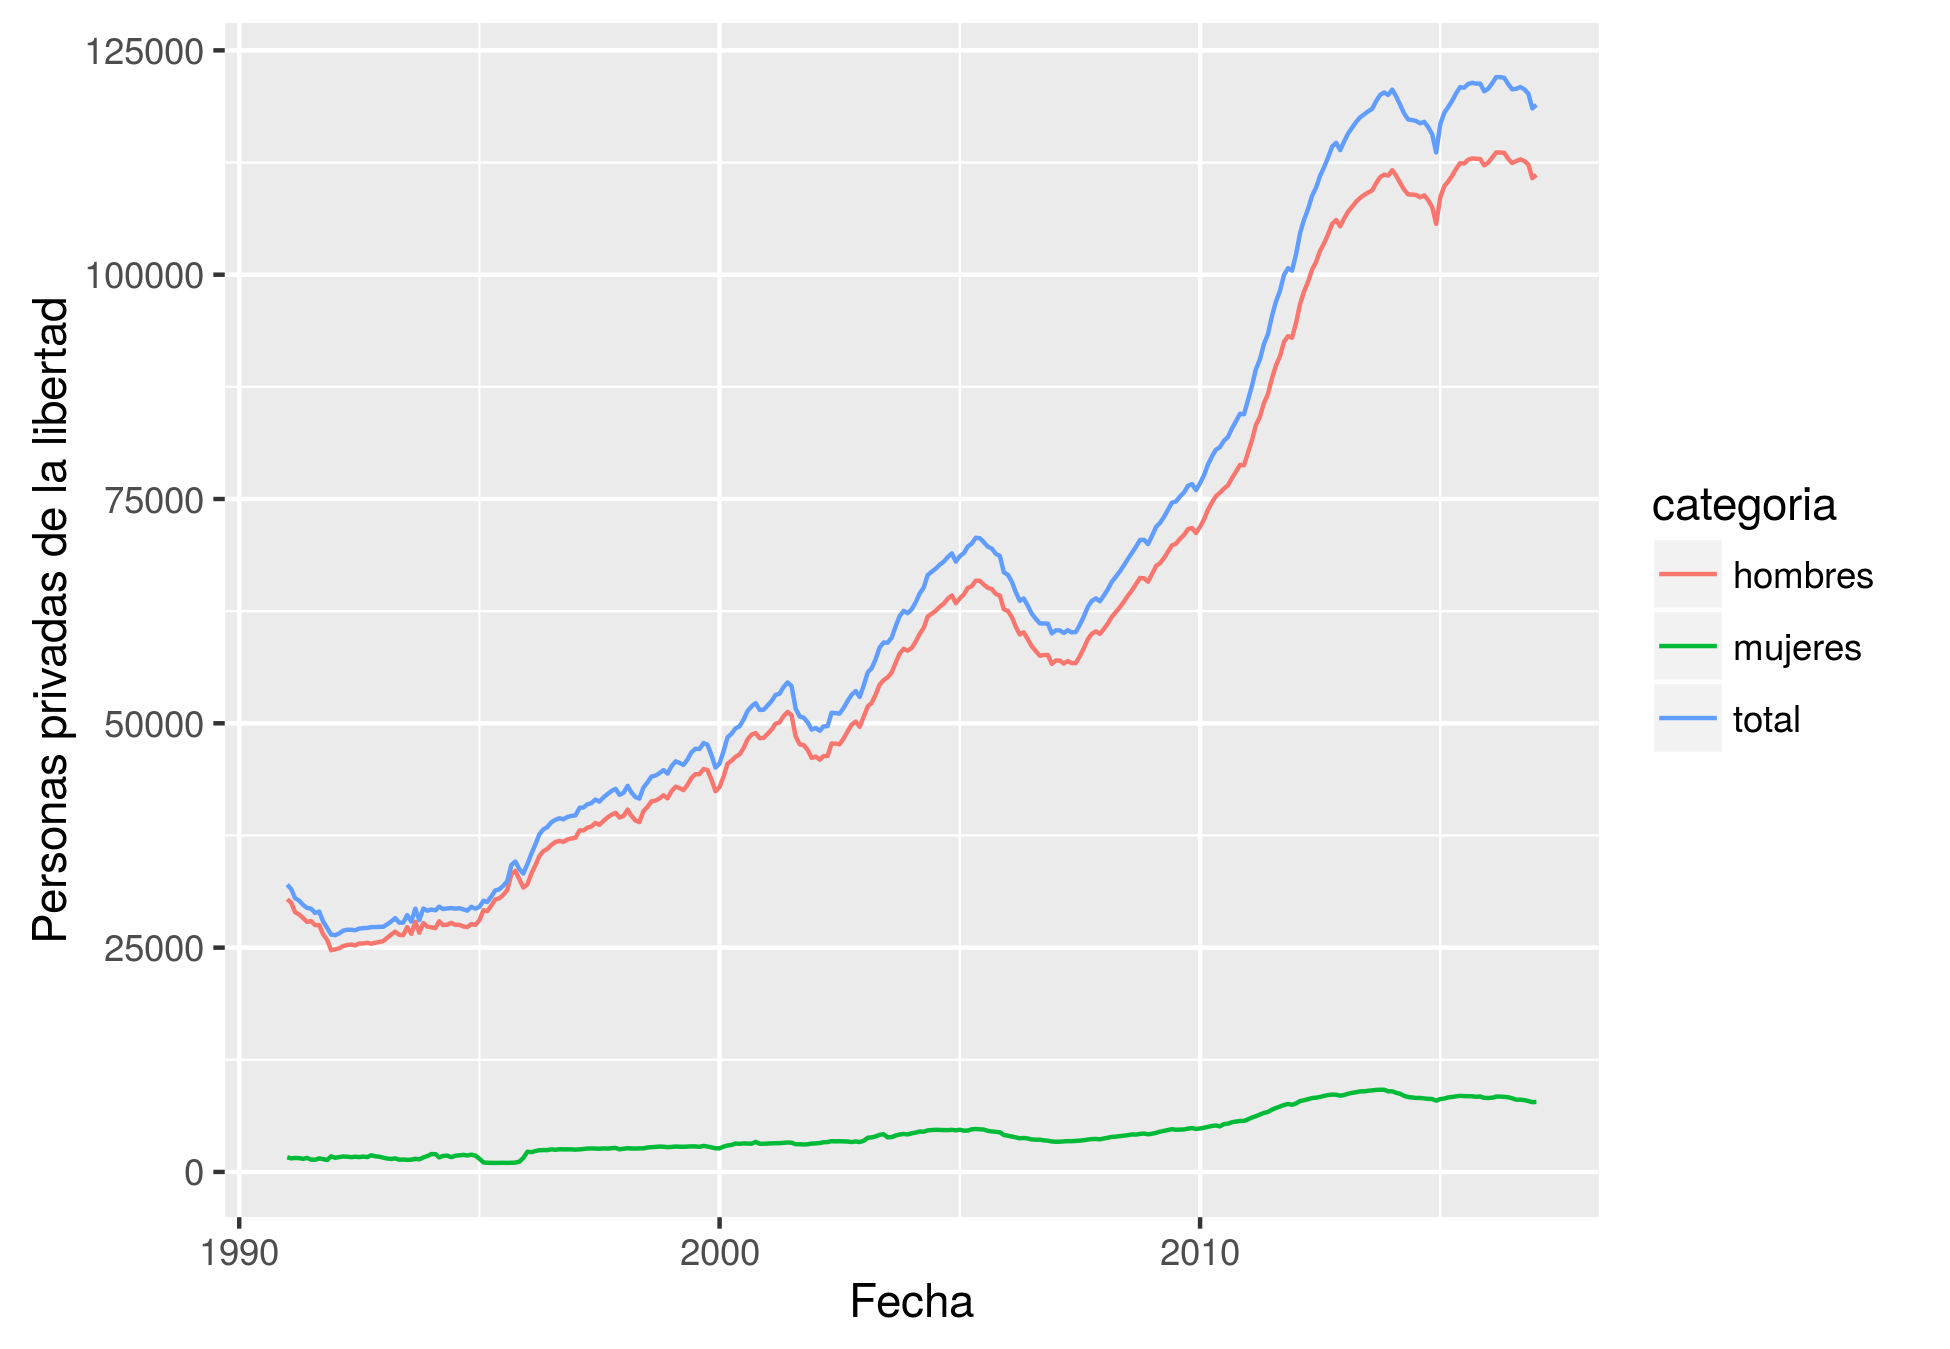
\includegraphics[width=10cm]{genero.png}
	\caption{Poblaci�n privada de la libertad 1991 - 2017} {Fuente: INPEC\\} {Elaboraci�n propia}
	\label{fig:genero}
\end{figure}

El incremento en la poblaci�n carcelaria podr�a tomarse como un efecto del crecimiento de la poblaci�n colombiana. Para validar este supuesto calculamos la tasa de encarcelamiento, que mide la cantidad de personas encarceladas por cada cien mil habitantes. Este indicador pas� de 92 personas por cada cien mil habitantes en enero de 1991 a 242 en enero de 2016. Tal incremento se puede ver tanto en hombres como en mujeres. Ver figura \ref{fig:tasas}. 


\begin{figure}[htb]
	\centering
	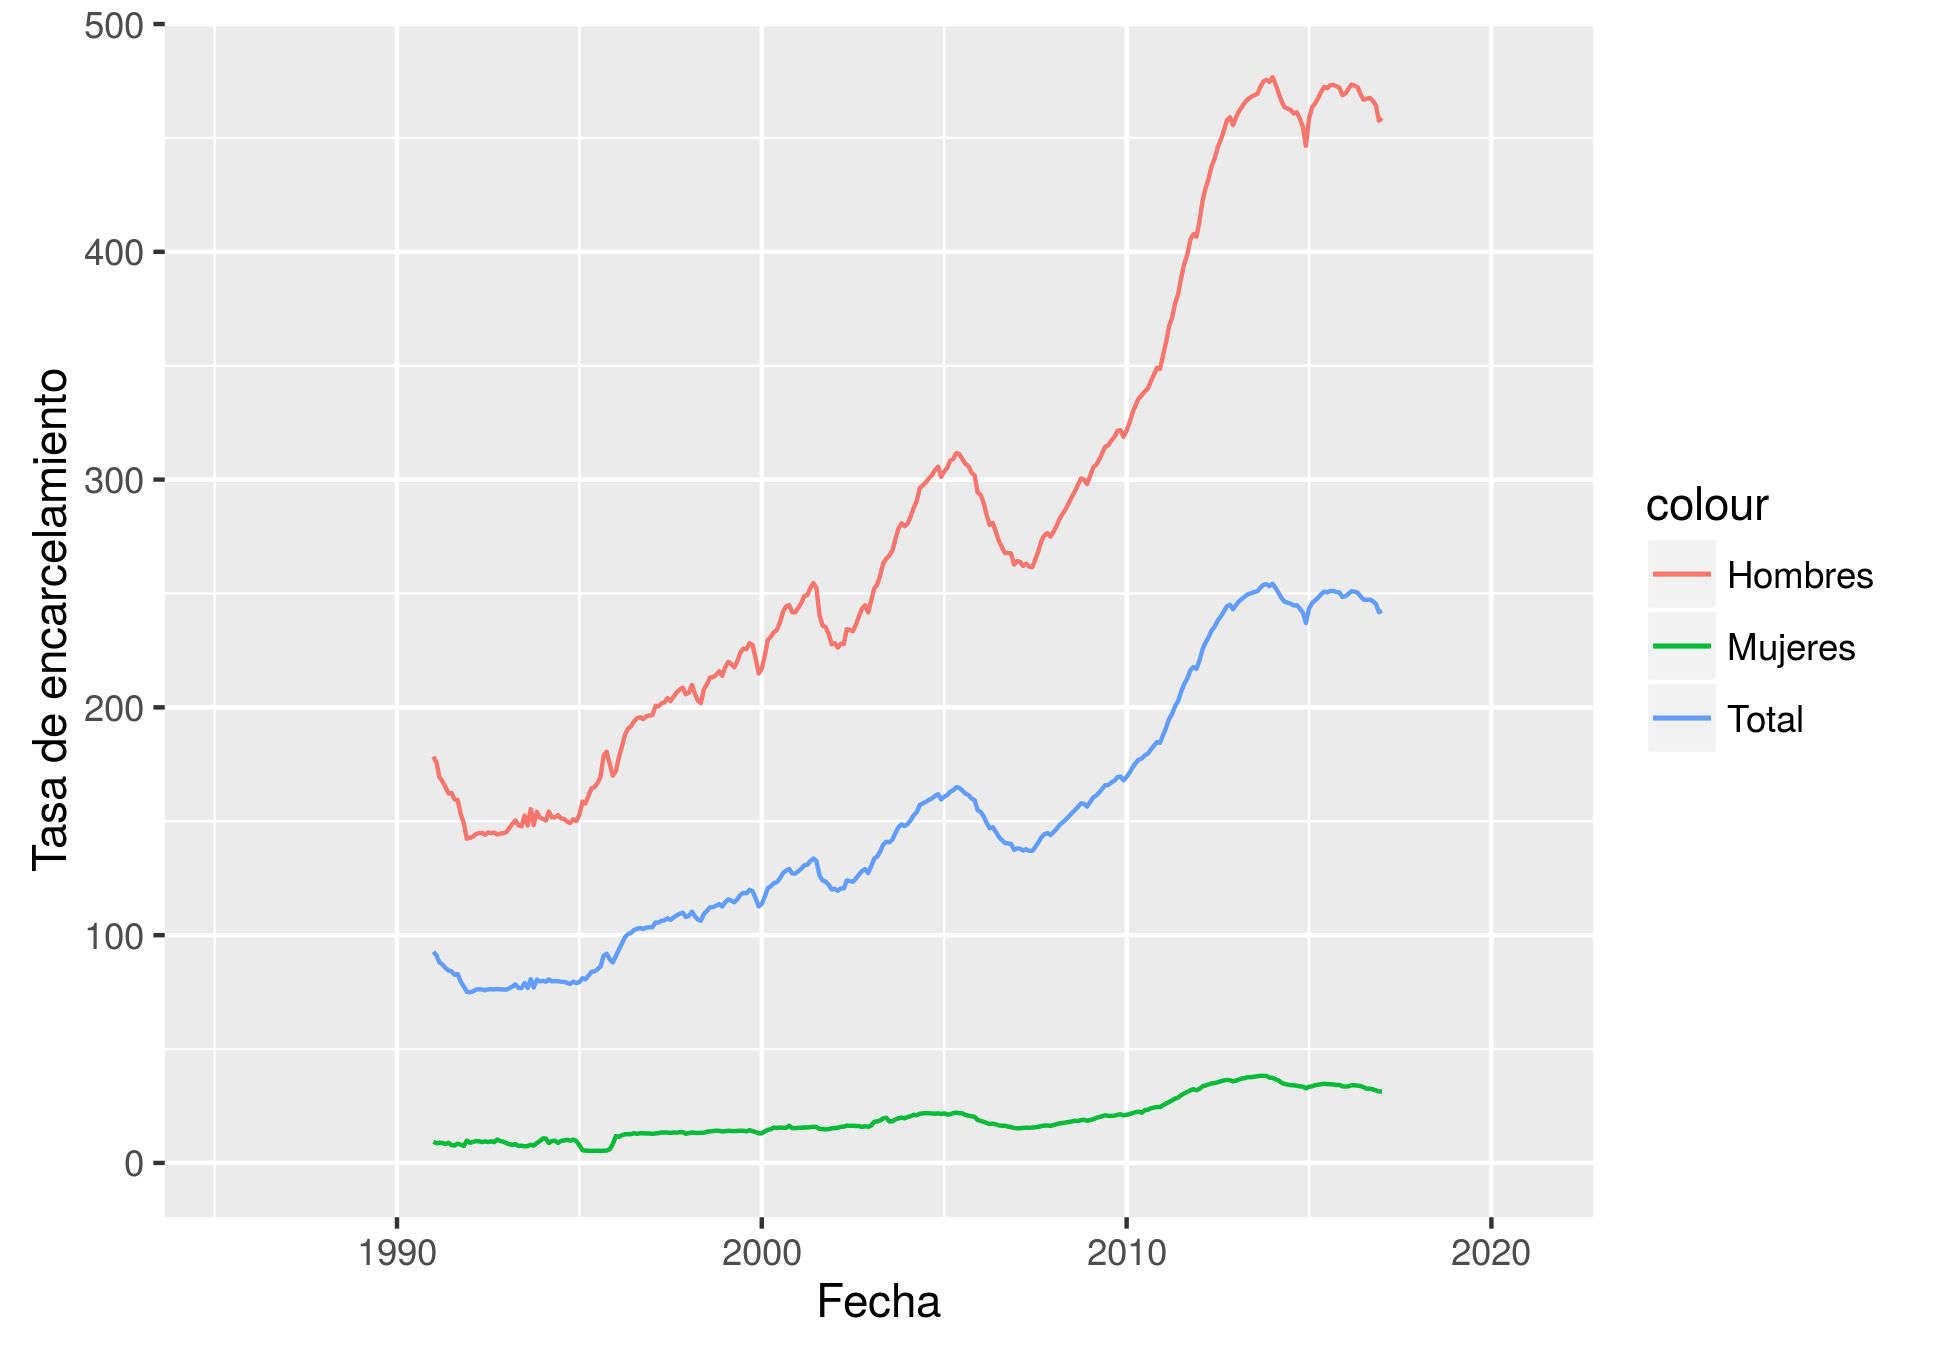
\includegraphics[width=10cm]{tasas}
	\caption{Tasa de encarcelamiento seg�n genero 1991 - 2017\\}{Fuente: INPEC\\} {Elaboraci�n propia}
	\label{fig:tasas}
\end{figure}

La tasa de encarcelamiento es un indicador que var�a seg�n la edad y genero, siendo m�s elevado en los hombres que en las mujeres y m�s algo en los hombres j�venes, que en los hombres mayores (cita pendiente).  Otra posible explicaci�n al cambio en la tasa de encarcelamiento es un cambio en la pir�mide poblacional en el periodo analizado. No obstante, no podemos confirmar o refutar esta hip�tesis pues la serie de tiempo, contenida en los datos de libre acceso no se encuentra desagregada por edad.

\section{El sistema penitenciario en Colombia}

La poblaci�n carcelaria se ve afectada por dos pol�ticas, la pol�tica penitenciaria, que determina las condiciones de privaci�n de la libertad y la pol�tica criminal que determina las causas de encarcelamiento y la duraci�n de las penas. \cite{DepartamentoNacionaldePlaneacion2015}

A la poblaci�n privada de la libertad antes del juicio se le denomina pobaci�n sindicada, y a aquellos que han sido juzgados y se encuentran cumpliendo la sentencia se les denomina poblaci�n condenada. La evoluci�n de la poblaci�n seg�n situaci�n jur�dica se puede observar en la figura \ref{fig:sit_jur}

\begin{figure}[htb]
	\centering
	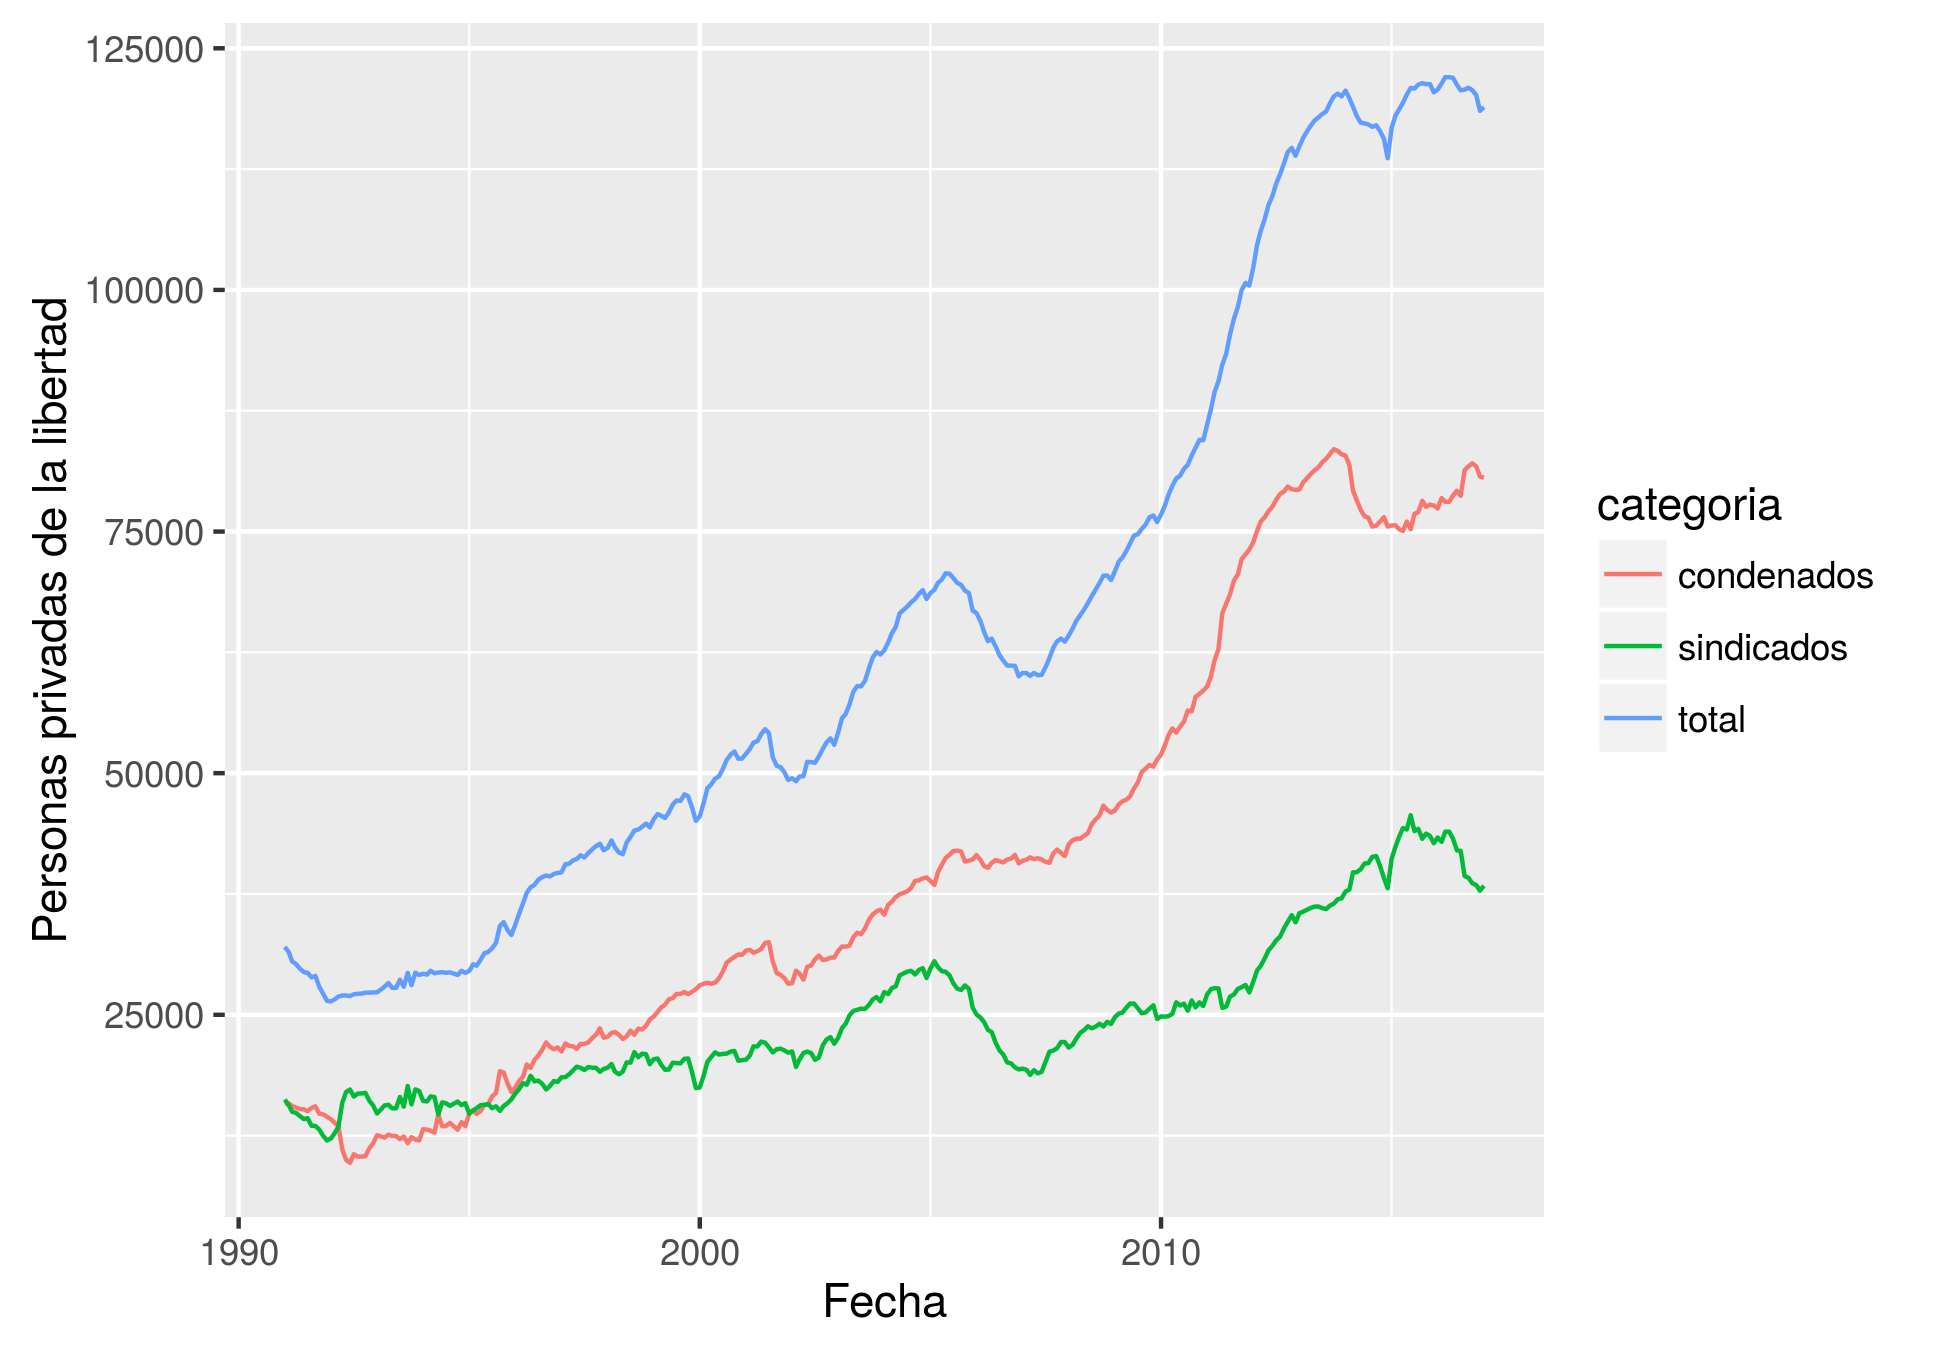
\includegraphics[width=10cm]{sit_jur.png}
	\caption{Poblaci�n carcelaria por situaci�n jur�dica\\} {Fuente: INPEC\\} {Elaboraci�n propia}
	\label{fig:sit_jur}
\end{figure}

\subsection{Identificaci�n del modelo}

Podemos modelar el sistema penitenciario de la siguiente manera:
%
\begin{equation}\label{Sindicados}
	S_t = S_{t-1} + \alpha {N_t} - \gamma S_{t-1}
\end{equation} 
%
\begin{equation}\label{Condenados}
	C_t = C_{t-1} - \omega C_{t-1} + \beta \gamma S_{t-1}
\end{equation} 
%
	$N_t$ = poblaci�n nacional en el periodo t \\
	$S_t$ = poblaci�n de sindicados en el periodo t\\
	$C_t$ = poblaci�n de condenados en el periodo t\\
	$\alpha$ = proporci�n de la poblaci�n libre que ingresa al sistema carcelario \\
	$\gamma$ = proporci�n de sindicados que es juzgada cada periodo \\
	$\beta$ = proporci�n de sindicados que han sido encontrados culpables durante el juicio	\\
	$\omega$ = proporci�n de condenados que cumplen su pena cada\\ periodo.
	
Y esto es un problema interesante porque no tengo las series de tiempo de la transici�n! 
    \chapter{Modelos SARIMA}

La estimaci�n de los modelos se realiza usando el paquete base del software R \cite{RCoreTeam2017}, y el paquete astsa \cite{Stoffer2014}, cuyo uso es discutido en detalle por Shumway \cite{Shumway}. 

En adelante nos referiremos a la funci�n de auctocorrelaci�n como ACF y a la funci�n de autocorrelaci�n parcial como PACF. 

\section{Identificaci�n del modelo}

% Variaci�n poblaci�n total, sindicada y condenada
\begin{figure}[H]
	\centering
	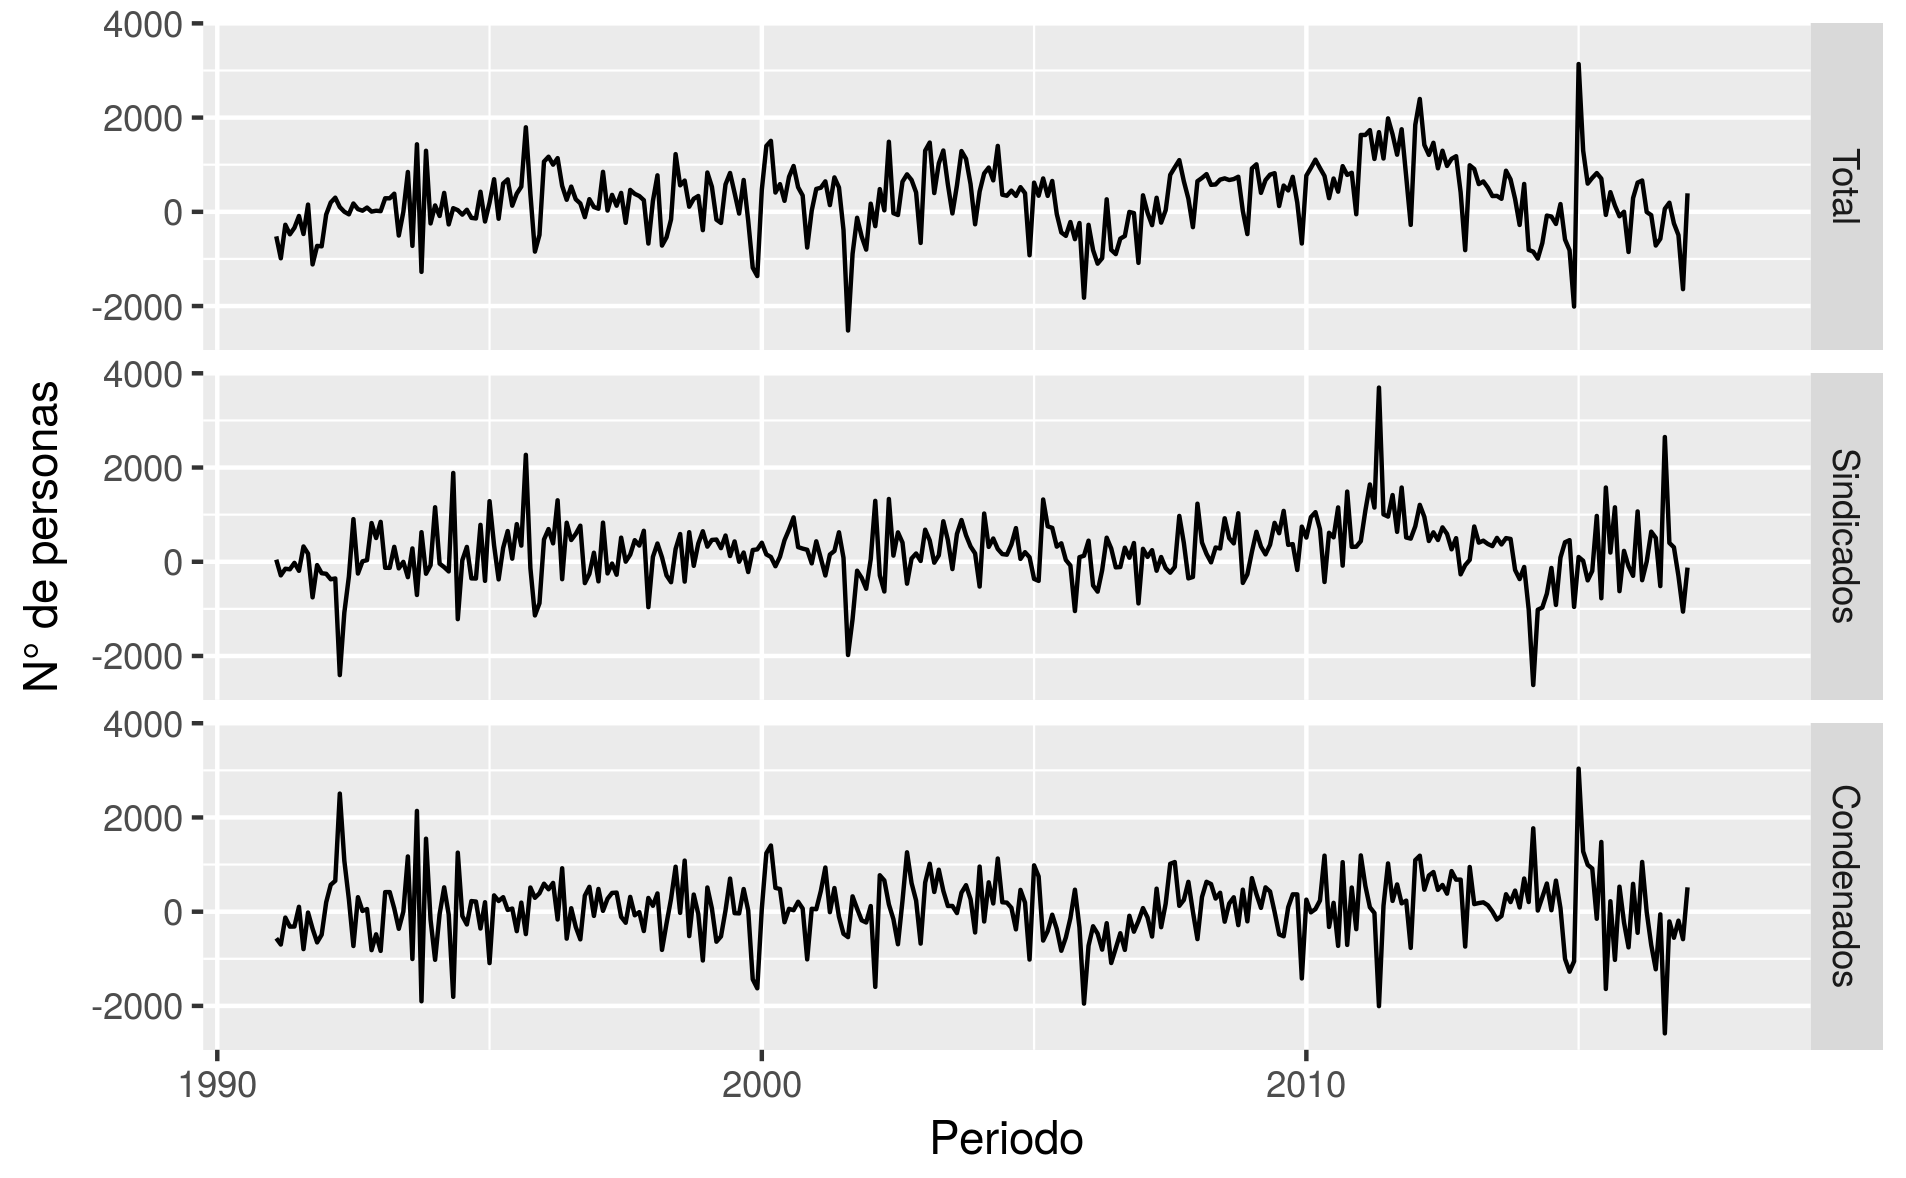
\includegraphics[width=0.7\linewidth]{variacion_intermensual}
	\caption[Variaci�n inter-mensual de poblaci�n carcelaria]{Variaci�n inter-mensual de poblaci�n carcelaria, sindicados y condenados}
	\label{fig:variacion_intermensual}
\end{figure}

Antes de realizar la proyecci�n de una serie de tiempo, es necesario identificar el modelo que explique adecuadamente su comportamiento. 

Aunque conocemos, por la estructura del proceso que genera los datos, que las series de tiempo de poblaci�n sindicada y condenada no son independientes, podemos simplificar la proyecci�n, trat�ndolas como independientes. En este caso, los modelos ARIMA y SARIMA resultan apropiados, pues permiten explicar separadamente cada observaci�n en funci�n del comportamiento hist�rico de la serie.

El cap�tulo anterior suger�a que la poblaci�n carcelaria, tanto sindicada como condenada, tiene una marcada tendencia al alza. En este caso una herramienta �til es mostrar gr�ficamente la variaci�n mes a mes de la poblaci�n. \ref{fig:variacion_intermensual}. Para tener una mejor estrucutura de an�lisis usamos la funci�n "decompose" de R base. 

La serie tiene un componente estacional marcado, con una reducci�n de la poblaci�n carcelaria en diciembre. La variabilidad del componente aleatorio es elevada. La tendencia parece tener cambios estructurales en algunos periodos, por ejemplo reducci�n de la poblaci�n carcelaria entre 2005-2007,  y 2012 - 2015, e incrementos de la poblaci�n de magnitud mayor al promedio entre 2008 y 2012.

La mayor parte de la variaci�n de la poblaci�n total se puede asociar con variaciones en a poblaci�n sindicada \ref{fig:variacion_mensual_sindicados_desc}. La poblaci�n condenada tiene una tendencia con una tendencia m�s estable.  \ref{fig:variacion_mensual_condenados_desc}

% Descomposici�n variaci�n poblaci�n total
\begin{figure}[H]
\centering
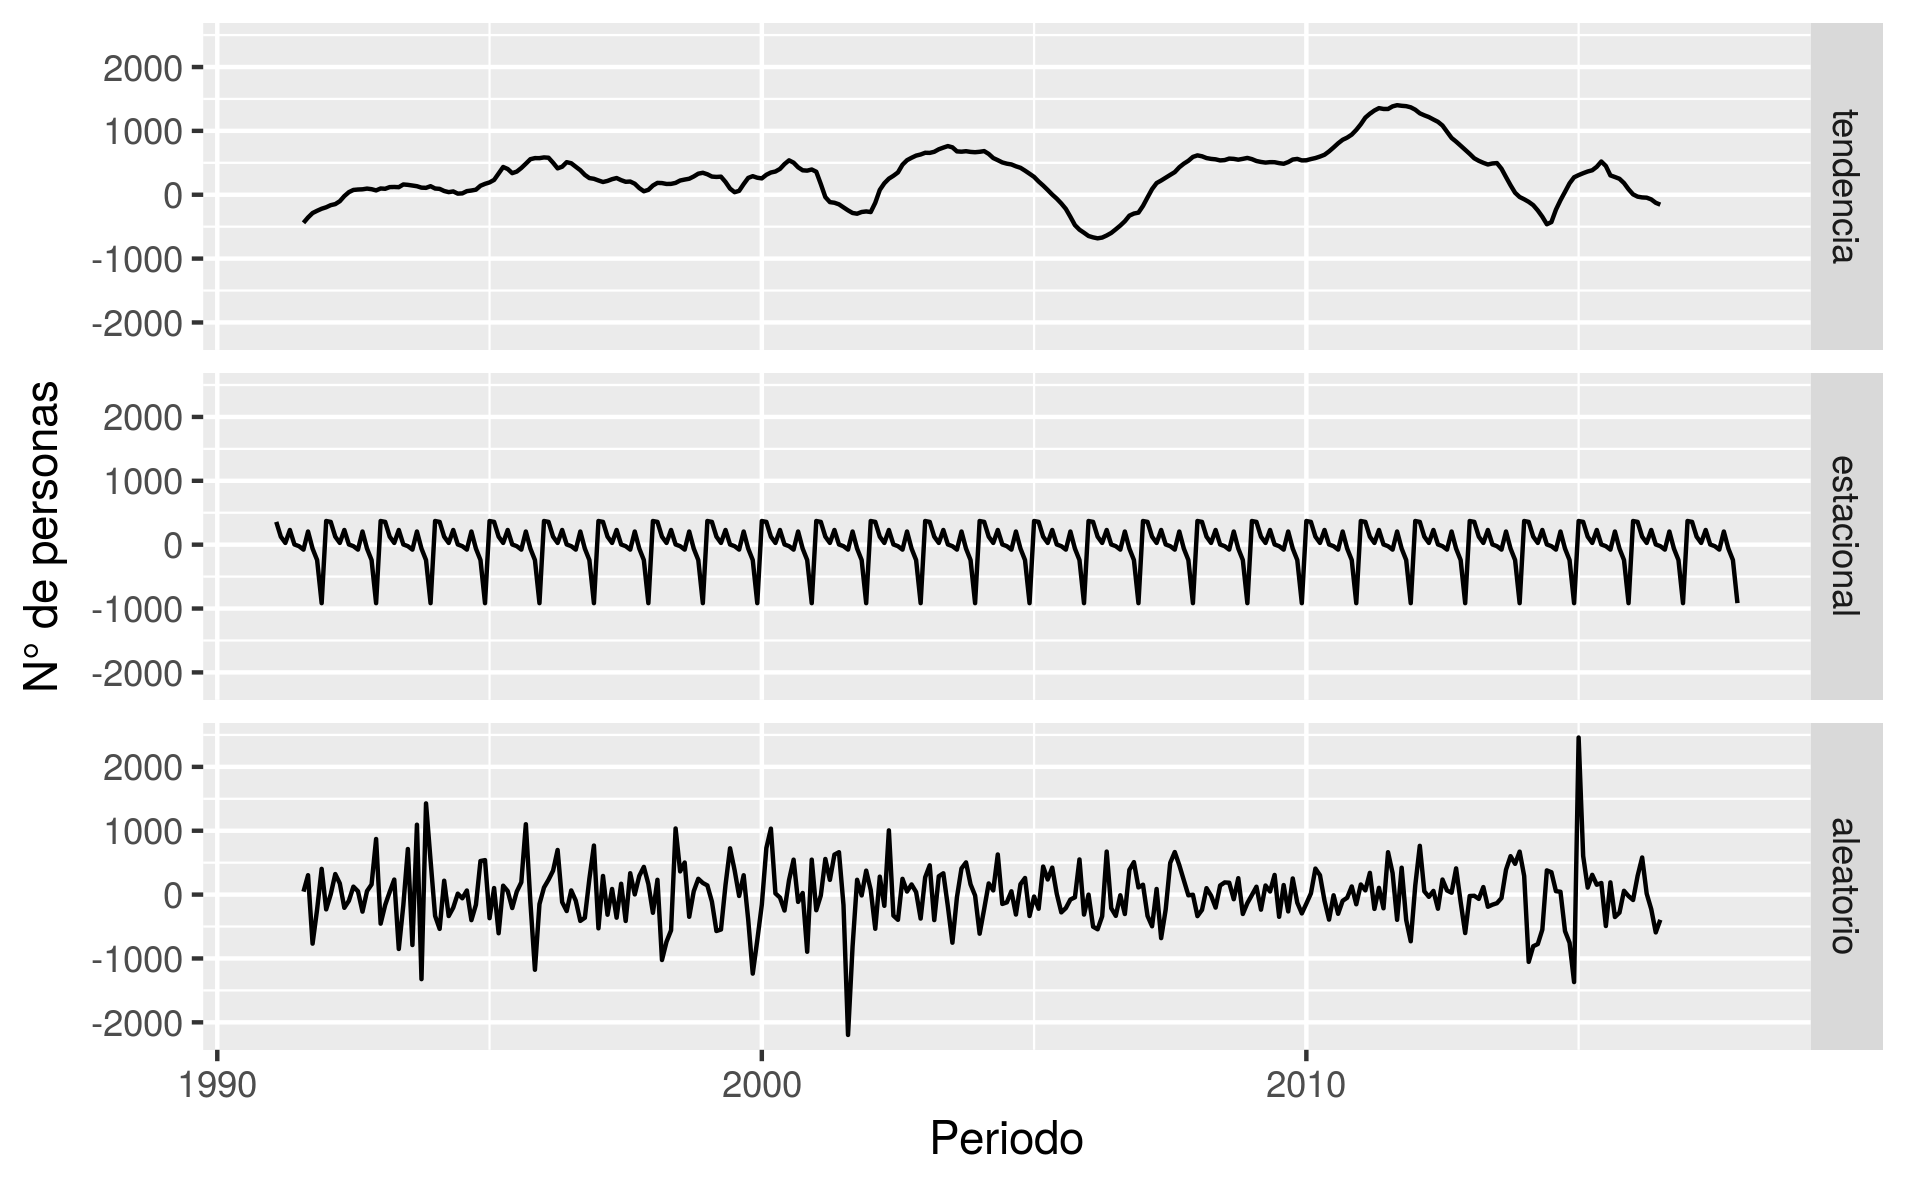
\includegraphics[width=0.7\linewidth]{variacion_mensual_total_desc}
\caption[Descomposici�n de la variaci�n inter-mensual de poblaci�n carcelaria total]{Variaci�n mensual de poblaci�n carcelaria descompuesta por tendencia, estacionalidad y componente aleatorio.}
\label{fig:variacion_mensual_total_desc}
\end{figure}

% Descomposici�n variaci�n poblaci�n sindicada
\begin{figure}[H]
	\centering
	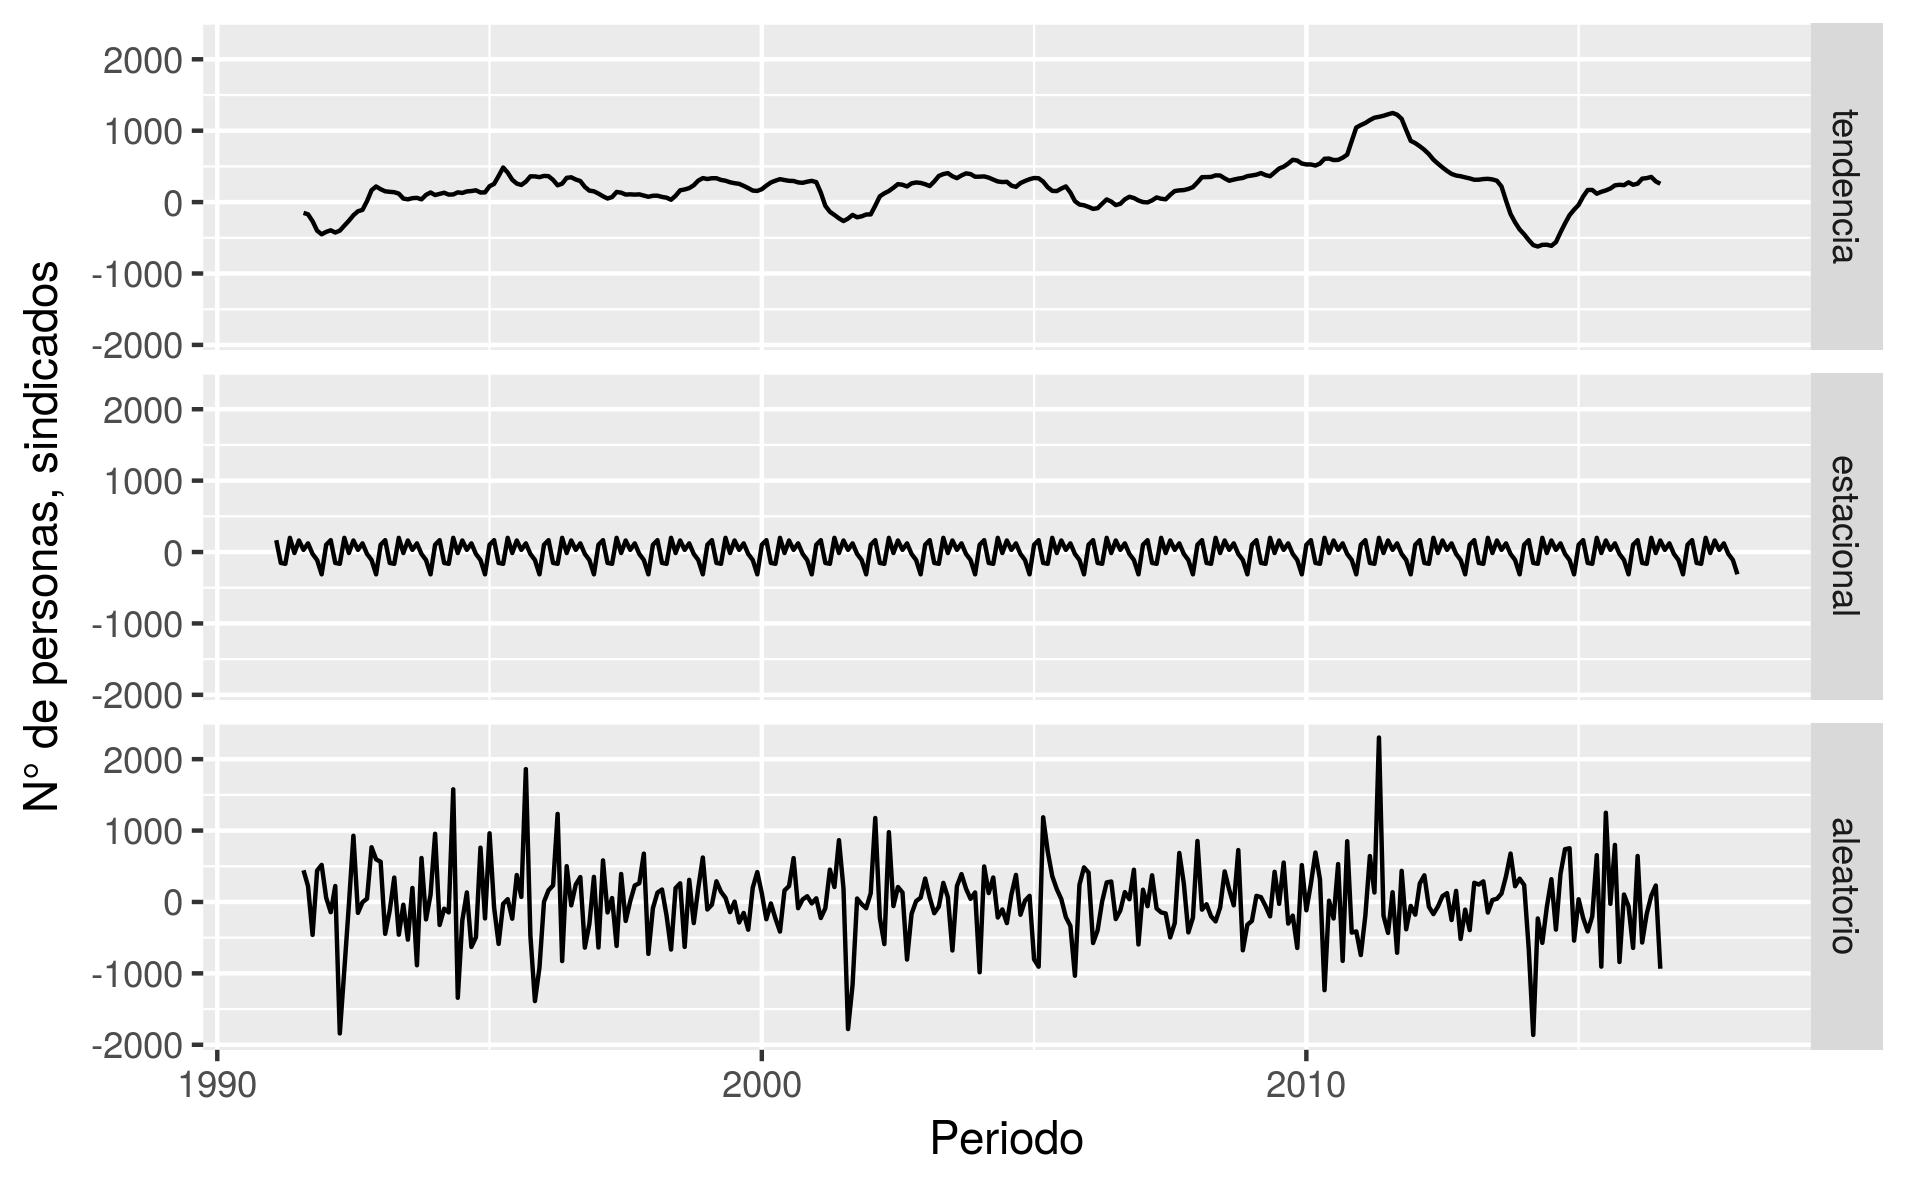
\includegraphics[width=0.7\linewidth]{variacion_mensual_sindicados_desc}
	\caption[Descomposici�n de la variaci�n inter-mensual de poblaci�n carcelaria total]{Variaci�n mensual de poblaci�n carcelaria sindicada,  descompuesta por tendencia, estacionalidad y componente aleatorio.}
	\label{fig:variacion_mensual_sindicados_desc}
\end{figure}

% Descomposici�n variaci�n poblaci�n condenada
\begin{figure}[H]
	\centering
	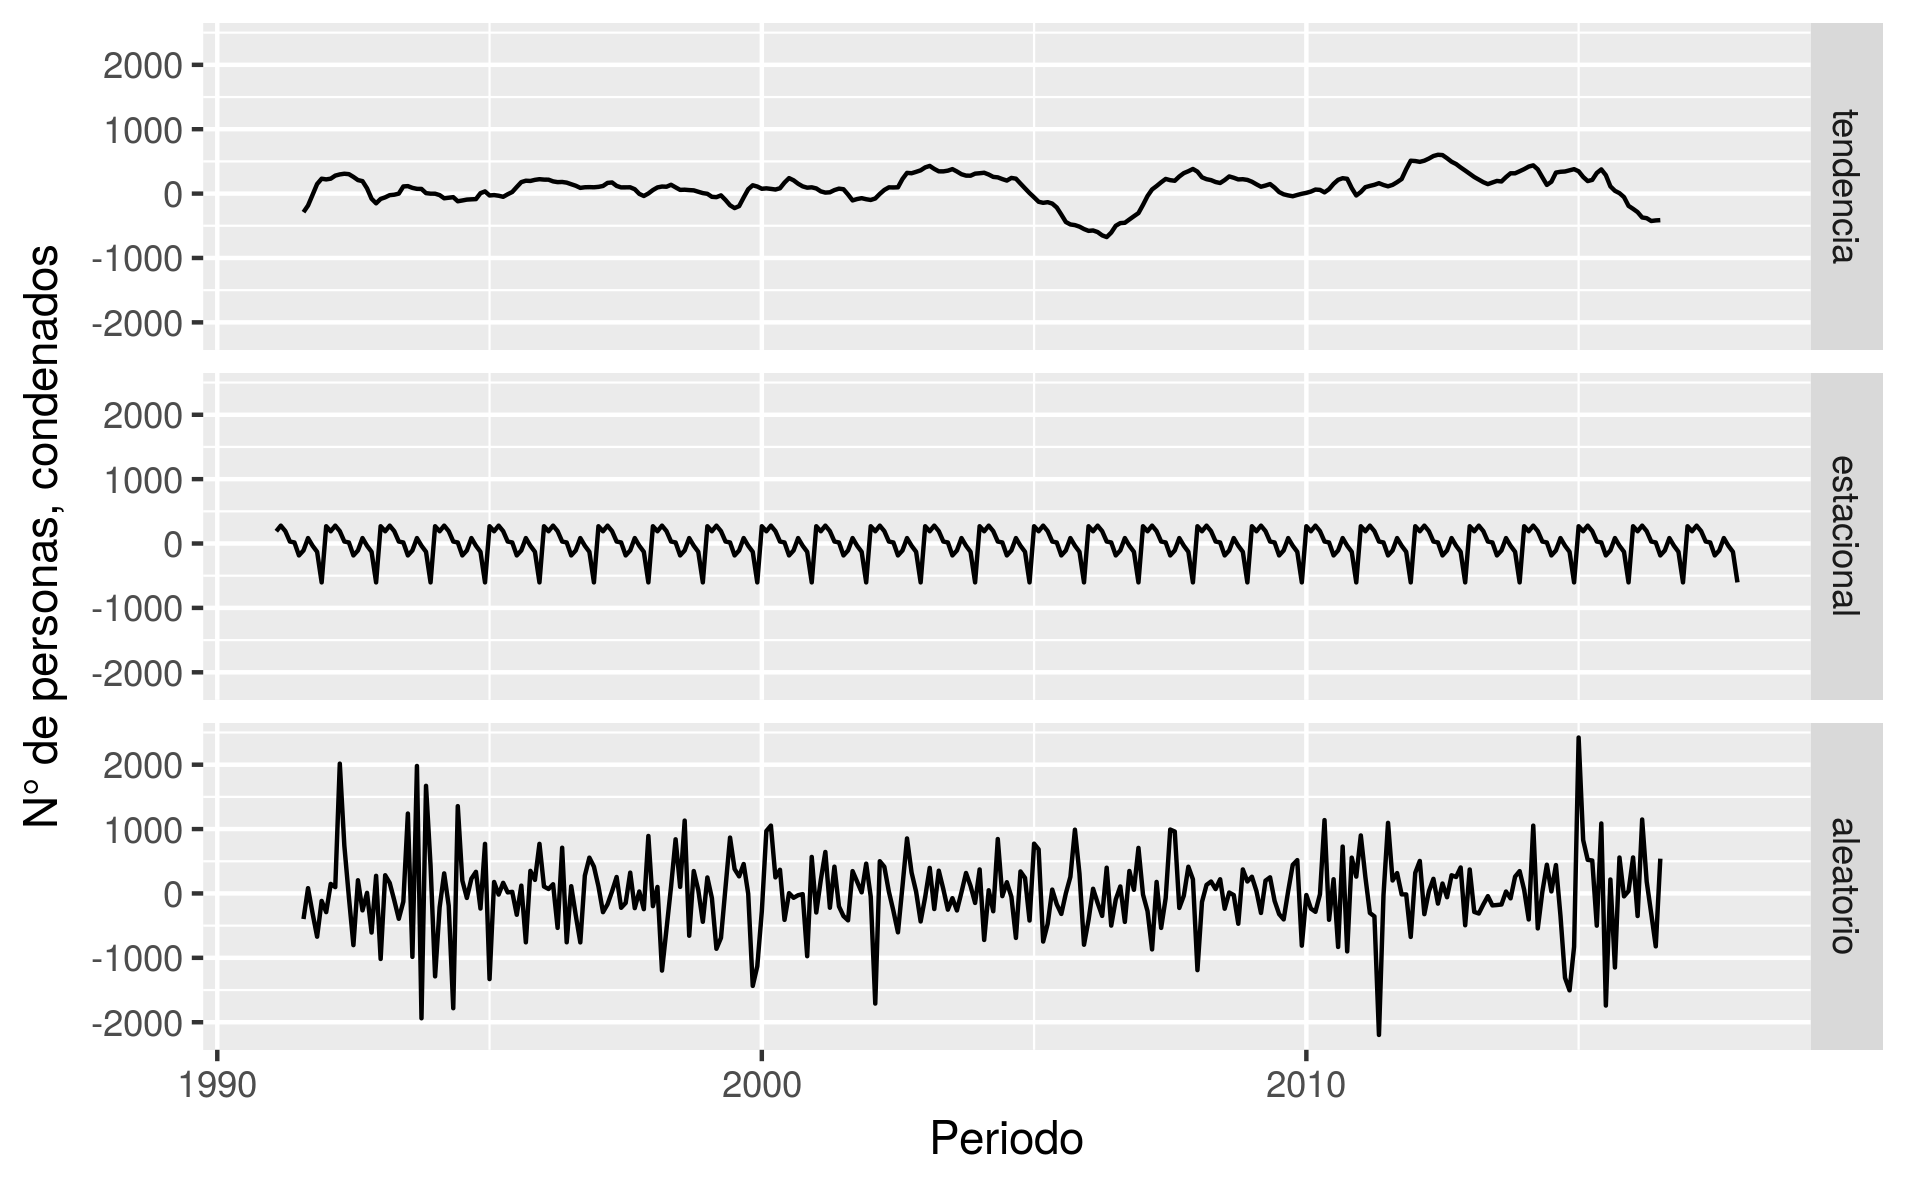
\includegraphics[width=0.7\linewidth]{variacion_mensual_condenados_desc}
	\caption[Descomposici�n de la variaci�n inter-mensual de poblaci�n carcelaria total]{Variaci�n mensual de poblaci�n carcelaria condenada,  descompuesta por tendencia, estacionalidad y componente aleatorio.}
	\label{fig:variacion_mensual_condenados_desc}
\end{figure}


Se trabaja sobre la diferencia de cada serie de tiempo con lag 1 y lag 12, al observar que la serie tiene un crecimiento sostenido entre 1991 y 2017, sugiriendo un proceso estocastico integrado. Sobre cada serie (poblaci�n total, poblaci�n sindicadda y poblaci�n condenada)  se realiza la funci�n de autocorrelaci�n y autocorrelaci�n parcial y se presenta en la figura \ref{fig:ACF_variacion_mensual}. Estas funciones son usadas como herramienta de diagn�stico, para intuir modelos adecuados en cada serie.

Con base en la tabla \ref{ARMA_ACF} se realiza una revisi�n del comportamiento de las series de poblaci�n carcelaria, poblaci�n sindicada y poblaci�n condenada.

% Pendiente traducir este fragmento
\begin{table}[H]
	\centering
	\caption{Comportamiento de la ACF y PACF en modelos ARMA(p,q) \cite{Shumway}}
	\label{ARMA_ACF}
	\begin{tabular}{lllll}
		\multicolumn{1}{|l|}{}              & \multicolumn{1}{c|}{\textbf{AR(p)}}       & \multicolumn{1}{c|}{\textbf{MA(q)}}       & \multicolumn{1}{c|}{\textbf{ARMA(p,q)}} &  \\ \cline{1-4}
		\multicolumn{1}{|l|}{\textbf{ACF}}  & \multicolumn{1}{l|}{Tails off}            & \multicolumn{1}{l|}{Cuts off after lag q} & \multicolumn{1}{l|}{Tails off}          &  \\ \cline{1-4}
		\multicolumn{1}{|l|}{\textbf{PACF}} & \multicolumn{1}{l|}{Cuts off after lag p} & \multicolumn{1}{l|}{Tails off}            & \multicolumn{1}{l|}{Tails off}          &  \\ \cline{1-4}
	\end{tabular}
\end{table}


\begin{figure}[H]
	\centering
	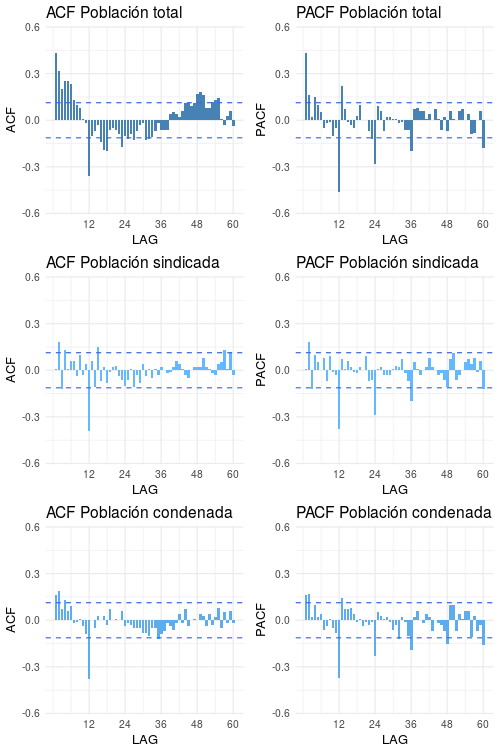
\includegraphics[width=0.7\linewidth]{ACF_var_pob}
	\caption[Autocorrelaci�n parcial de la variaci�n inter-mensual]{Autocorrelaci�n parcial de la variaci�n inter-mensual de la poblaci�n}
	\label{fig:ACF_variacion_mensual}
\end{figure}

\subsection{Poblaci�n total}

La tabla \ref{ARMA_ACF} presenta una gu�a para la interpretaci�n de la ACF y la PACF. En la \ref{fig:ACF_variacion_mensual} podemos observar que tanto la ACF como la PACF decaen lentamente. La APCF decae progresivamente en los meses 12, 24, 36, mientra que la ACF se corta en el lag 24, lo que sugiere que el proceso es un promedio m�vil de orden 1 en el componente estacional.

En este caso una primera estimaci�n se realiza para la proyecci�n de la poblaci�n total como SARIMA(1,1,1,0,0,1)


\subsection{Poblaci�n sindicada}

En la \ref{fig:ACF_variacion_mensual} podemos observar que la ACF decae lentamente, mientras la PACF cae por debajo del error luego del lag 1. La APCF decae progresivamente en los meses 12, 24, 36, mientra que la ACF se corta en el lag 12, lo que sugiere que el proceso es un promedio m�vil de orden 1 en el componente estacional.

En este caso una primera estimaci�n se realiza para la proyecci�n de la poblaci�n sindicada como SARIMA(1,1,1,0,0,1)

\subsection{Poblaci�n condenada}

El comportamiento de la ACF y la PACF es similar al de la poblaci�n sindicada, sugiriendo el mismo modelo: SARIMA(1,1,1,0,0,1).

\section{Estimaci�n de par�mtetros}
El proceso de estimaci�n se realizar� para cada serie por separado, luego se validar� la efectividad de incluir m�s par�metros, usando como criterio de comparaci�n el BIC. A modo informativo se usa la funci�n auto.arima del paquete forecast, para seleccionar el modelo con menor AIC. \cite{Hyndman2017}  
 \cite{Hyndman2008} 
 
\subsection{Poblaci�n total}

\subsection{Poblaci�n sindicada}

\subsection{Poblaci�n condenada}


\section{Proyecci�n}

\subsection{Poblaci�n total}

\subsection{Poblaci�n sindicada}

\subsection{Poblaci�n condenada}

\section{Conclusiones}

Al usar un ARIMA
    \chapter{PROYECCIONES CON MODELOS ESTADO ESPACIO}

\section{Marco te�rico}

\section{Identificaci�n del modelo}

\section{Simulaci�n Monte-Carlo}

\section{Estimaci�n de par�metros}

\section{Proyecciones 2017 - 2020}

\section{Conclusiones}
\appendix
    \chapter{Gr�ficas adicionales}

\begin{figure}[htb]
 \centering
 
\includegraphics[width=10cm]{small_escudo_color}
 \caption{Escudo oficial de la UN a color dise�ado por el Maestro Francisco Duarte.}
 \label{fig:escudo_color}
\end{figure}


\begin{table}
\centering
\caption{Unidades de \TeX.}
\begin{tabular}{l|l}\hline
\verb"mm" & mil�metro $\approx$ 1/25 pulgada \\
\verb"cm" & cent�metro = 10 mm \\
\verb"in" & pulgada $\approx$ 25 mm \\
\verb"pt" & punto $\approx$ 1/72 pulgada $\approx$ 1/3 mm \\
\verb"em" & aprox. el ancho de una m en el tipo actual \\
\verb"ex" & aprox. la altura de una x en el tipo actual \\\hline
\end{tabular}
\end{table}

\begin{table}
\centering\renewcommand{\arraystretch}{2}
\caption{Tama�os de los tipos de fuentes \LaTeX.}
 \begin{tabular}{ll|ll}\hline
{\tiny\verb"\tiny"} & {\tiny letra diminuta}
& {\large\verb"\large"} & {\large letra grande} \\
{\scriptsize\verb"\scriptsize"} & {\scriptsize letra muy peque�a}
& {\Large\verb"\Large"} & {\Large letra mayor} \\
{\footnotesize\verb"\footnotesize"} & {\footnotesize letra bastante peque�a}
& {\LARGE\verb"\LARGE"} & {\LARGE muy grande} \\
{\small\verb"\small"} & {\small letra peque�a}
& {\huge\verb"\huge"} & {\huge enorme} \\
\verb"\normalsize" & letra normal
& {\Huge\verb"\Huge"} & {\Huge la mayor} \\\hline
 \end{tabular}
\end{table}





\backmatter
    \conclusion{conclusiones}
    \futurework{trabajofuturo}
    \glossary{glosario}
\nocite{*}
    \bibliography{references}
    %\printindex
\end{document}
